\section{Notes}

\newpage

\subsection{VC Dimension}

An alternative approach is to write down the VC dimension by using
an instance space and a concept class as given
in \cite{computational-learning-theory}.

\begin{lemma}
    Let $X = \left\{ x_1, ..., x_n \right\} \subset \mathbb{R}^d \times \mathbb{R}_{>0}$
    be the instance space consisting of $n$ points with their last
    coordinate being positive.
    The concept class of interest, $\mathcal{C}$ over $X$, is given as follows:
    \begin{equation*}
        \mathcal{C} = \left\{ \{x \in X:\ f_{\beta, r}(x) \geq 0 \} \ |\ \beta \in \mathbb{R}^d, r \geq 0 \right\},
    \end{equation*}
    with
    \begin{equation*}
        f_{\beta, r}(x) = x_{d+1} \cdot g\left(\sum_{i=1}^d x_i \beta_i\right) - r
    \end{equation*}
    and
    \begin{equation*}
        g(x) = -\log \Phi(-x).
    \end{equation*}
    The VC dimension of $\mathcal{C}$ is equal to the VC dimension of the
    range space induced by
    $\mathcal{F}^w_{probit} = \{ w_i g(z_i \beta) \ | \ i \in [n] \}$,
    $Z \in \mathbb{R}^{n \times d}$, $w \in \mathbb{R}^n_{>0}$.
\end{lemma}

There a few different strategies that can be used to find an upper
bound on the VC dimension of $\mathcal{C}$, as shown by the following
lemmas.
The first one is a simple upper bound for finite concept classes:

\begin{lemma}
    Let $X$ be an instance space and $\mathcal{C}$ be a concept class
    over $X$.
    If the cardinality of $\mathcal{C}$ can be bounded by $m$, i.e.
    $|\mathcal{C}| \leq m$, then $VCdim(\mathcal{C}) \leq log(m)$.
\end{lemma}

The next lemma partitions the concept class into smaller classes,
for each of which the VC dimension can be bounded:

\begin{lemma}
    Let $X$ be an instance space and $\mathcal{C}$ be a concept class
    over $X$.
    Let $\mathcal{C}_1, ..., \mathcal{C}_k$ be a partition of $\mathcal{C}$
    into $k$ disjoint subsets, i.e.
    $\mathcal{C} = \bigcup_{i=1}^k \mathcal{C}_i$ and
    $\mathcal{C}_i \cap \mathcal{C}_j = \emptyset\ \forall i \neq j$.
    Then, $VCdim(\mathcal{C}) \leq \sum_{i=1}^k VCdim(\mathcal{C}_i)$.
\end{lemma}
\begin{proof}
    For the sake of contradiction, assume there was a set $S \subseteq X$
    of size $|S| > \sum_{i=1}^k VCdim(\mathcal{C}_i)$ that is shattered by
    $\mathcal{C}$. If $S$ is shattered by $C$, every subset of $S$ must also
    be shattered by $C$.
    Consider the intersections $T_i = \bigcup_{c \in \mathcal{C}_i} S \cap c$.
    Every $T_i$
    is a subset of $S$ and $S = \bigcup_{i=1}^k T_i$.
    Since $S$ is shattered by $\mathcal{C}$,
    every $T_i$ must be shattered by $\mathcal{C}_i$.
    We assumed that $|S| > \sum_{i=1}^k VCdim(\mathcal{C}_i)$.
    It follows that there exists a $T_j$ with $T_j > VCdim(\mathcal{C}_j)$.
    Since $T_j$ is also shattered by $\mathcal{C}_j$, this is a contradiction,
    which concludes the proof.
\end{proof}

A result in~\cite{vc-dimension-partition} suggests an even smaller upper bound:
\begin{lemma}[\cite{vc-dimension-partition}]
    Let $X$ be an instance space and $\mathcal{C}$ be a
    concept class over $X$.
    Let $\mathcal{C} = \bigcup_{i=1}^k \mathcal{C}_i$
    and $VCdim(\mathcal{C}_i) \leq m$.
    If $k$ is bounded by a polynomial function of $m$,
    then $VCdim(\mathcal{C}) \leq 3m$.
\end{lemma}

Instead of partitioning the concept class, we could also partition the
instance space and obtain a similar bound:

\begin{lemma}
    \label{lemma:instance-space-partition}
    Let $X$ be an instance space and $\mathcal{C}$ be a concept class
    over $X$.
    Let $X_1, ..., X_k$ be a partition of $X$ into $k$ disjoint subsets, i.e.
    $X = \bigcup_{i=1}^{k} X_i$ and
    $X_i \cap X_j = \emptyset\ \forall i \neq j$.
    Let $\mathcal{C}_i = \left\{ X_i \cap c\ |\ c \in \mathcal{C} \right\}$
    be a concept class over $X_i$ for all $i \in [k]$.\\
    Then, $VCdim(\mathcal{C}) \leq \sum_{i=1}^k VCdim(\mathcal{C}_i)$.
\end{lemma}
\begin{proof}
    Again, assume there existed a set $S \subseteq X$ of size
    $|S| > \sum_{i=1}^k VCdim(\mathcal{C}_i)$ that is shattered
    by $\mathcal{C}$.
    $S$ can be partitioned into disjoined subsets $T_i = S \cap X_i$, with
    $\bigcup_{i=1}^k T_i = S$.
    Every $T_i$ must be shattered by $\mathcal{C}_i$.
    Since we assumed that $|S| > \sum_{i=1}^k VCdim(\mathcal{C}_i)$,
    there exists a $T_j$ with $|T_j| > VCdim(C_j)$ which is also
    shattered by $C_j$. This contradiction concludes the proof.
\end{proof}

\newpage

\subsection{New idea for VC dimension proof}

\begin{lemma}
    Let
    \begin{equation*}
        h_{\beta, r}(x) =
        \begin{cases}
            1 \ \textup{if} \quad x_{d+1} \cdot g\left( \sum_{i=1}^d x_i \beta_i \right) - r \geq 0 \\
            0 \ \textup{else}
        \end{cases}
    \end{equation*}
    Be a function from $\mathbb{R}^{d+1}$ to $\{0, 1\}$ with parameters
    $\beta \in \mathbb{R}^d$ and $r \in \mathbb{R}_{\geq 0}$ with
    \begin{equation*}
        g(x) = \log\left( \frac{1}{1 - \Phi(x)}\right),
    \end{equation*}
    \begin{equation*}
        \Phi(x) = \frac{1}{\sqrt{2 \pi}} \int_{-\infty}^x e^{-\frac{1}{2}z^2}dz\ .
    \end{equation*}
    Let
    \begin{equation*}
        H = \left\{ x \mapsto h_{\beta, r}(x) \ |\ \beta \in \mathbb{R}^{d},\ r \in \mathbb{R}_{\geq 0} \right\}
    \end{equation*}
    be the hypothesis class determined by $h$. Then, the VC dimension of $H$ is \ldots
\end{lemma}
\begin{proof}
    Let $S = \sum_{i=1}^d x_i \beta_i$. We show that $h$ can be computed in
    $t$ steps as follows:
    \begin{gather*}
        x_{d+1} \cdot g\left( S \right) - r                            \geq 0                                      \\
        \iff  \log\left( \frac{1}{1 - \Phi(S)}\right)                        \geq \frac{r}{x_{d+1}}                      \\
        \iff  \frac{1}{1 - \Phi(S)}                                          \geq \exp\left(\frac{r}{x_{d+1}}\right)     \\
        \iff  1 - \Phi(S)                                                    \leq \exp\left(-\frac{r}{x_{d+1}}\right)    \\
        \iff  \Phi(S)                                                        \geq 1 -\exp\left(-\frac{r}{x_{d+1}}\right) \\
        \iff  \frac{1}{\sqrt{2 \pi}} \int_{-\infty}^S e^{-\frac{1}{2}z^2}dz  \geq 1 -\exp\left(-\frac{r}{x_{d+1}}\right) \\
        \iff   \int_{-\infty}^S e^{-\frac{1}{2}z^2}dz  \geq \sqrt{2 \pi}\left(1 -\exp\left(-\frac{r}{x_{d+1}}\right)\right) \\
    \end{gather*}
\end{proof}

\newpage

\subsection{Online Leverage Scores}

The leverage scores of a matrix $A \in \mathbb{R}^{n \times d}$
are given by $l_i = a_i^T (A^TA)^{-1}a_i$~\cite{online-row-sampling}.
According to~\cite{online-row-sampling}, we can obtain overestimates
of these scores by using only a subset of the rows in $A$ to compute them.

Let $A_j$ be a matrix that contains only the first $j$ rows of $A$.
It follows that the the estimated leverage score
$\tilde{l}_j = a_j^T (A_j^TA_j)^{-1}a_j$ is an overestimate of $l_j$.
In a recent paper by~\cite{tensor-factorization}, it was shown that
the sum of these overestimates can be bounded regardless of how
the rows in $A$ are ordered:
\begin{lemma}[\cite{tensor-factorization}]
    \begin{equation*}
        \sum_{i=1}^n \tilde{l}_j \in O(d + d \log \lVert A \rVert - \min_{i \in [n]} \lVert a_i \rVert)
    \end{equation*}
\end{lemma}

Next, we show how a simple algorithm that computes $\tilde{l}_j$ in an
online manner (passing row by row over the data stream)
can be constructed requiring only $\mathcal{O}(d^2)$ of working memory.
The idea is to only keep the matrix $A_j^TA_j \in \mathbb{R}^{d \times d}$
in memory and update it
for every new row $a_{j+1}$ using a rank one update
$A_{j+1}^TA_{j+1} = A_j^TA_j + a_{j+1} \cdot a_{j+1}^T$.
See~\cite{matrix-computations} for more on matrix multiplication using
outer products. The algorithm is given in algorithm~\ref{algo:online-leverage-scores}.

\begin{algorithm}
    \DontPrintSemicolon
    \KwIn{Matrix $A \in \mathbb{R}^{n \times d}$}
    \KwOut{Online leverage scores $\tilde{l}_i$ for all $i \in [n]$}
    Initialize $M_0 = 0^{d \times d}$ \;
    \ForEach{$a_i := i\textup{'th row vector of }A$, $a_i \in \mathbb{R}^d$}{
        $M_i = M_{i-1} + a_i \cdot a_i^T$ \;
        $\tilde{l}_i = a_i^T M_i^\dagger a_i$ \;
    }
    \KwRet{$\tilde{l}_i,\ i \in [n]$}
    \caption{Online Leverage Scores\label{algo:online-leverage-scores}}
\end{algorithm}

\subsection{Probit Regression}

\begin{lemma}
    Let $g(z) = -\log \Phi(-z)$. Then it holds for all $z \geq 0$ that:
    $$
        \frac{1}{2} z^2 \leq g(z)
    $$
\end{lemma}
\begin{proof}
    The following relationship holds for all $z \geq 1$:
    \begin{align*}
        \Phi(-z) & = \frac{1}{\sqrt{2 \pi}} \int_{-\infty}^{-z} \exp{ \left(-\frac{1}{2} x^2 \right)} dx       \\
                 & \leq \frac{1}{\sqrt{2 \pi}} \int_{-\infty}^{-z} -x \exp{ \left(-\frac{1}{2} x^2 \right)} dx \\
                 & = \frac{1}{\sqrt{2 \pi}} \exp{\left( -\frac{1}{2} z^2 \right)}                              \\
                 & \leq \exp{\left( -\frac{1}{2} z^2 \right)}                                                  \\
    \end{align*}
    We therefore have for $z \geq 1$:
    $$
        e^{g(z)} = e^{-\log \Phi(-z)} = \frac{1}{\Phi(-z)} \geq e^{\frac{1}{2} z^2}
    $$
    Since $\exp( \cdot )$ is a monotonically increasing function,
    it follows that $g(z) \geq \frac{1}{2}z^2$ for all $z \geq 1$.

    \noindent{}Let us now turn to the case when $0 \leq z \leq 1$.
    Both $g(z)$ and $\frac{1}{2}z^2$ are monotonically increasing
    and continuous functions for $0 \leq z \leq 1$.
    Together with the fact that $g(0) > \frac{1}{2}$ it follows
    for all $0 \leq z \leq 1$ that
    $$
        g(z) \geq g(0) > \frac{1}{2} = \max_{0 \leq z \leq 1} \frac{1}{2} z^2 \geq \frac{1}{2} z^2
    $$
    which concludes the proof.
\end{proof}

\begin{lemma}
    Let $g(z) = -\log \Phi(-z)$. Then it holds for all $z \geq 2$ that:
    $$
        g(z) \leq z^2
    $$
\end{lemma}
\begin{proof}
    We first show that $\Phi(-z) \geq \frac{1}{\sqrt{2 \pi}} \frac{z}{z^2 + 1} e^{-\frac{1}{2} z^2}$
    for all $z \geq 0$.
    In order to prove this lower bound, we define
    $h(z) = \Phi(-z) - \frac{1}{\sqrt{2 \pi}} \frac{z}{z^2 + 1} e^{-\frac{1}{2} z^2}$
    and show that $h(z)$ is positive for all $z \geq 0$.
    The derivative $h'(z) = -\sqrt{\frac{2}{\pi}} \frac{e^{-\frac{1}{2} z^2}}{(z^2 + 1)^2}$ is
    negative for all $z$, so $h(z)$ is a monotonically decreasing function.
    Also, it clearly holds that $h(0) > 0$ and
    $\lim_{z \rightarrow \infty} h(z) = 0$. It follows that $h(z) \geq 0$
    for all $z > 0$ which proves the lower bound.

    In the next step, we use this result to show that $e^{z^2} \cdot \Phi(-z) \geq 1$
    for all $z \geq 2$:
    \begin{align*}
        e^{z^2} \cdot \Phi(-z) & \geq e^{z^2} \frac{1}{\sqrt{2 \pi}} \frac{z}{z^2 + 1} e^{-\frac{1}{2} z^2}                           \\
                               & = e^{\frac{1}{2} z^2} \frac{1}{\sqrt{2 \pi}} \frac{z}{z^2 + 1}                                       \\
                               & = e^{\frac{1}{2} z^2} \frac{1}{\frac{4}{3}\left( z^2 + 1 \right)} \frac{\frac{4}{3} z}{\sqrt{2 \pi}} \\
                               & \geq \frac{e^{\frac{1}{2} z^2}}{\frac{4}{3}\left( z^2 + 1 \right)}                                   \\
                               & \geq \frac{e^{\frac{1}{2} z^2}}{e^{\frac{1}{2} z^2}}                                                 \\
                               & = 1
    \end{align*}
    From this it follows directly that $\frac{1}{\Phi(-z)} \leq e^{z^2}$
    and thus we have for all $z \geq 2$:
    $$
        e^{g(z)} = e^{-\log \Phi(-z)} = \frac{1}{\Phi(-z)} \leq e^{z^2}
    $$
    Since $\exp{\left( \cdot \right)}$ is monotonically increasing, the claim
    that $g(z) \leq z^2$ for all $z \geq 2$ follows as a direct consequence.

    The ideas for these proofs are based on the work in~\cite{gaussian_bounds}.
\end{proof}

\subsection{Lower Bounds}

\begin{theorem}
    Let $X \in \mathbb{R}^{n \times 2}$, $y \in \{-1, 1\}^n$ be
    an instance of probit regression.
    Any coreset $C \in \mathbb{R}^{k \times 2}$ of $X$, $y$
    for probit regression consists of
    at least $k \in \Omega\left(\frac{n}{\log{n}}\right)$ points.
\end{theorem}
\begin{proof}
    We first show how such a coreset could be used in a
    communication protocol for the INDEX communication game
    to encode a message.
    Since there exists a lower bound on the minimum
    message length of the INDEX game (see~\cite{index}),
    we can use it to derive a lower bound on the
    coreset size.
    The same technique was also used in~\cite{on-coresets} to find
    lower bounds for coresets of logistic regression and is here slightly
    adapted for probit regression.

    The INDEX game consists of two players, Alice and Bob.
    Alice is given a random binary string $x \in \{0, 1\}^n$ of $n$ bits
    and Bob is given an index $i \in [n]$.
    The goal is for Alice to send a message to Bob that allows
    Bob to obtain the value $x_i$ of Alice's binary string $x$.
    It was shown in~\cite{index}, that the minimum length of a message
    sent by Alice that still allows Bob to obtain $x_i$ with
    constant probability is in $\Omega(n)$ bits.
    We will now see how a coreset for probit regression can be used
    to encode such a message.

    The first step is for Alice to convert her binary string $x$ into
    a set $P$ of two-dimensional points as follows:
    For each entry $x_j$ of her binary string where $x_j = 1$, she adds
    a point $p_j = \left( \cos{\left(2 \pi \frac{j}{n}\right)},
        \sin{\left(2 \pi \frac{j}{n}\right)} \right)$
    to her set $P$ and labels it with $1$.
    As we can see, all of these points are on the unit circle and all
    of them are labeled with $1$.
    Next, she uses these points to construct a coreset for probit regression
    $C \in \mathbb{R}^{k \times 2}$ of $P$
    and sends it to Bob. We will later see, how
    large the size $k$ of this coreset must be, so that Bob can still
    obtain $x_i$ with constant probability.

    As soon as Alice's coreset $C$ arrives at Bob, Bob can use it to
    obtain the value of $x_i$.
    To do this, Bob first adds two new points
    $q_1 = \left( \cos{\left(2 \pi \frac{i - 0.5}{n}\right)},
        \sin{\left(2 \pi \frac{i - 0.5}{n}\right)} \right)$
    and
    $q_2 = \left( \cos{\left(2 \pi \frac{i + 0.5}{n}\right)},
        \sin{\left(2 \pi \frac{i + 0.5}{n}\right)} \right)$
    to the set and labels both points with $-1$ (see figure~\ref{fig:index}).
    Next, he uses his points $q_1$ and $q_2$ together with the coreset $C$ to
    obtain a solution for the corresponding probit regression problem.
    He can then use the value of the cost function to determine the value
    of $x_i$ like this:

    Since Alice only added a point $p_j$ to her set if $x_j = 1$, both
    of his points $q_1$ and $q_2$ are linearly seperable from Alice's points if
    the value of $x_i = 0$, i.e. Alice didn't add a point for $x_i$.
    In this case, the value of the cost function tends to zero.
    If, on the other hand, Bob's new points $q_1$ and $q_2$ can't be linearly
    seperated from the other points, it means that Alice added a point
    for $x_i = 1$. In this case, there must be at least one
    misclassification and the value of the cost function is at least
    $g(0) = \log(2)$.
    Since coresets can be used to obtain $(1 + \epsilon)$-approximation
    of the objective function, Bob can use this case distinction to
    determine the value of $x_i$.

    There is one special case that has to be dealt with in order for this
    protocol to work. If Alice's coreset only consists of the single point
    $p_i$, Bob's points $q_1$ and $q_2$ could still be linearly seperated
    although Alice added $p_i$.
    The workaround to this is simple though:
    Bob can always just add two more
    points at the locations of $p_{i-1}$ and $p_{i+1}$ and label them with 1.
    Now, $q_1$ and $q_2$ can only be linearly seperated from the
    other points if and only if Alice didn't add a point $p_i$.

    Let us now see how large the size $k$ of Alice's coreset must be
    for this protocol to work with constant probability.
    In~\cite{index} it was shown, that the minimum length of a message
    that Alice must send is in $\Omega(n)$ bits.
    Since each of the points that Alice created can be encoded in
    $\log(n)$ space, it follows from the lower bound that
    $\Omega(n) \subseteq \Omega(k \log(n))$, so $k$ must be in
    $\Omega\left(\frac{n}{\log(n)}\right)$.

    We can conclude that if there existed a $(1 + \epsilon)$-coreset
    for probit regression with size $k \in o\left(\frac{n}{\log(n)}\right)$,
    it would contradict the minimum message length of
    INDEX, which proves the claim.
\end{proof}

\begin{figure}
    \centering
    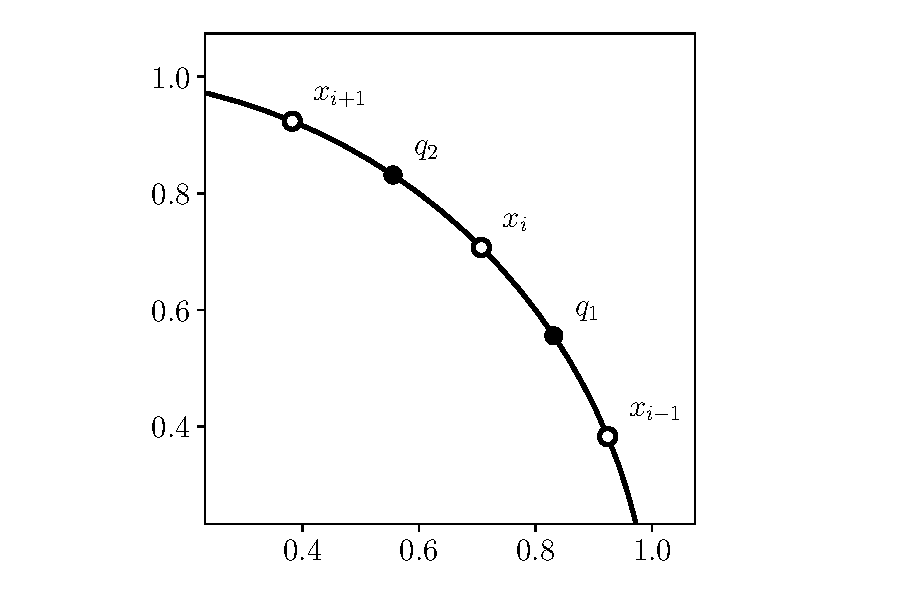
\includegraphics[width=0.8\textwidth]{figures/index.pdf}
    \caption{Bob places two points $q_1$ and $q_2$ in such a way
        on the unit circle, that they can be linearly seperated from the other
        points if and only if Alice didn't place a point at $p_i$.}
    \label{fig:index}
\end{figure}
